\chapter{Analyse}

Ziel der Arbeit ist es, dass ein Anwender die in der HsH-Datenbank vorhandenen Bilddaten in eine Menge von $k$ verschiedenen Gruppen einteilen kann, um so semantische Informationen über die Bilder zu gewinnen. Das $k$ kann hierbei vom Anwender vorgegeben werden um verschiedene Gruppen zu erhalten und so unterschiedliche Informationen in Bildern zu entdecken. 
In diesem Rahmen sollen zwei Methoden miteinander verglichen werden, die eine Gruppierung von Bildern auf Basis von sogenannten Feature-Deskriptoren ermöglichen.  Die so entstandenen Modelle erlauben es weitere Bilder zu \textit{labeln}, d.h. die Gruppe zu bestimmen, der sie angehören. Eine wesentliche Eigenschaft die der Deskriptor aufweisen sollte, ist affine Invarianz. Verschiedene Objekte oder Merkmale die auf mehreren Bildern vorhanden sind, besitzen selten die gleiche Position, daher sollten Rotation, Skalierung und Translationen berücksichtigt werden können. Gegenwärtig ist aber noch kein Deskriptor vorhanden, der eine Einbeziehung aller möglichen Umstände realisiert. Eine Reihe von geeigneten und verbreiteten Deskriptoren wird im Kapitel \nameref{extraction} vorgestellt und diskutiert.
Ein Vergleich von Bildern anhand von Features ist nicht unmittelbar möglich. Die Feature-Vektoren weisen viele Komponenten auf, was eine effiziente Berechnung nicht möglich macht. Aus diesem Grund werden zwei unüberwachte Lernverfahren vorgestellt: Zum Einen wird das Bag of Visual Words Modell behandelt, zum Anderen der Autoencoder. Beide Modelle bilden die erhobenen Feature-Vektoren auf einen Raum mit weniger Dimensionen ab, um so eine effizientere Berechnung der \textit{Labels} zu ermöglichen. Da, je nach gewünschtem Modell, zum Aufbauen desselben Tausende bis Millionen von Features verarbeitet werden müssen, wird bei der Betrachtung der beiden Ansätze geprüft, wie eine Beschleunigung der Berechnung durch parallele Verarbeitung erzielt werden kann. Gerade bei großen Datenmengen und einer enormen Datenparallelität können Probleme durch GPUs um ein vielfaches schneller gelöst werden, als durch CPUs.

\todo{cuda besser einführen, kurze cuda Sektion?}

\section{Feature Deskriptoren}
\label{extraction}

Feature Deskriptoren enthalten Informationen von charakteristischen Bereichen in Bildern. Feature Deskriptoren kodieren weitaus mehr als nur die geometrische Position von Pixeln: Es wird beispielsweise die Beleuchtung und teilweise affine Invarianz berücksichtigt. In der Literatur finden sich verschiedene Ansätze, die je nach Einsatzgebiet unterschiedliche Stärken besitzen. Nachfolgend werden einige Feature Deskriptoren vorgestellt, die verbreitete Anwendung durch ihre praktischen Erfolge erzielt haben. Für die weitere Verarbeitung der Features ist es erstrebenswert, dass ihre Darstellung möglichst kompakt ist. Deskriptoren werden als Vektoren von Zahlen kodiert, die abhängig vom Verfahren Informationen über einen Pixel und seine Nachbarschaft oder auch ein ganzes Bild enthalten. Je größer die Anzahl der Einträge eines Vektors, desto größer wird der Speicherbedarf und Rechenaufwand. Neben einer kompakten Darstellung werden daher in der Praxis weitere Verfahren verwendet, um die Anzahl der Komponenten eines Vektors weiter zu reduzieren.

\todo{Under construction - auch die folgenden Deskriptoren}

\subsection{Local Binary Patterns}

Der Local Binary Pattern (LBP) Deskriptor erzeugt aus einem Bild eine Reihe Bitstrings als Deskriptoren. Die Länge der Bitstrings hängt hier von der verwendeten Größe der Nachbarschaft eines Pixel ab. Original wurde eine $3 \times 3$ Nachbarschaft verwendet, was zu einer Länge von acht führt (nur die Nachbarschaft wird kodiert). Für jeden Pixel wird nun bestimmt ob seine Intensität kleiner oder größer im Vergleich zu einem Schwellwert ist. Abhängig vom Ergebnis wird eine 0 oder 1 kodiert. Im Fall der $3 \times 3$ Nachbarschaft ergibt dies $2^8$ mögliche verschiedene Bitstrings, sodass der resultierende Featurevektor 256 Komponenten aufweist. LBP wurden um Invarianz gegenüber Rotationen und die Verarbeitung von Farbbildern erweitert. Durch die Entwicklung dieser Methode wurden vor allem im Bereich der Gesichtserkennung wesentliche Fortschritte gemacht \cite{lbp2002}.

\subsection{Spatial Envelope}

Einen ganz anderen Ansatz haben Torralba und Olivia \cite{mts2001} verfolgt: Statt Objekte durch lokale Features zu beschreiben, werden globale Eigenschaften betrachtet. Das Bild wird in einem Raum mit wenig Dimensionen abgebildet, dem sogenannten \textit{Spatial Envelope}. Die Autoren nutzen hier wahrnehmbare Dimensionen wie Natürlichkeit und Offenheit um den Raum zu definieren. Eine hohe Natürlichkeit weist zum Beispiel auf das Bild einer Landschaft hin: Hier kommen in der Regel kaum gerade vertikale und horizontale Linien vor, im Gegensatz zu Bildern, die von Menschen angefertigt wurden.  Bilder die in einer semantischen Kategorie Ähnlichkeiten aufweisen, liegen dann nah beieinander. Dieses Modell hat sich vor allem bewährt um eine Umgebung bzw. Landschaft zu klassifizieren. 

\subsection{Histogram of Oriented Gradients}

Der Histogram of Orientied Gradients (HOG) Deskriptor beschreibt die Features als Histogramm der Richtung der Gradienten eines Bildes. Da sich Gradienten eignen um Kanten in Bildern zu erkennen, wird so die Form der Objekte eines Bildes erkannt. Dalal und Triggs \cite{hog2005} entwickelten und nutzten diesen Verfahren bereits 2005, mit großem Erfolg, um Menschen in Bilder zu erkennen. Obwohl beispielsweise SIFT auch ein lokales Histogramm um einen \textit{keypoint} berechnet, werden beim HOG hingegen die Features des ganzen Bildes (bzw. Bereiches) berechnet, nicht nur von Nachbarschaften. Das Verfahren zur Gewinnung eines HOG ist im Grundlagenkapitel unter \ref{sec:hog} beschrieben. 

\subsection{SIFT}

Der SIFT-Deskriptor trifft keine speziellen Annahmen über die vorliegenden Objekte

\subsection{Bewertung der Deskriptoren}

In der Literatur und Praxis hebt sich von allen Deskriptoren der SIFT-Deskriptor am meisten ab. Zwar gibt es für spezielle Anwendungsfälle geeignetere Deskriptoren, wie beispielsweise den LBP-Deskriptor für die Erkennung von Passanten, doch SIFT ist bis heute der beste \glqq Allrounder\grqq. Insofern eignet sich SIFT vor allem, wenn nicht bekannt ist, allgemeine Inhalte in einer Bildmenge vorliegen bzw. wenn mehr als eine spezielle Objektart berücksichtigt werden muss. Generell funktionieren die im folgenden vorgestellten Modelle mit jeder Art von (Bild-)Deskriptor: Die Modelle arbeiten genau aus diesem Grund nicht direkt mit den Bilddaten, sondern den Deskriptoren. Bei eben diesen handelt es sich lediglich um Vektoren aus dem Raum $\mathbb{R}^d$, wobei die Dimensionalität $d$ des Raums und damit die Anzahl der Elemente des Vektors abhängig vom Verfahren sind. Dies schränkt aber nicht die generelle Machbarkeit ein, sondern wirkt sich auf die Laufzeit bzw. den Speicherbedarf aus. Da für die vorliegenden Bilddaten der HsH keine speziellen Annahmen getroffen werden können, wird für die Gewinnung der Features das SIFT-Verfahren und somit auch das Histogram of Oriented Gradients verwendet. 

\section{Lernverfahren}

Ein System, dass ein Lernverfahren implementiert, wird genutzt um Muster in Datenströmen zu entdecken. Hierfür wird das System mit Trainingsdaten angelernt, um diese zu beurteilen und daraus Muster zu gewinnen. Wenn dieser Vorgang abgeschlossen ist, kann der Lernalgorithmus auf die eigentlichen Daten angewendet werden. In der Literatur wird zwischen verschiedene Lernmethoden unterschieden, die geläufigsten sind unüberwachtes und überwachtes Lernen:

\begin{itemize}
	\item \textbf{Überwachtes Lernen (supervised Learning)} Ein Lehrer ist erforderlich, der überprüft, ob die Ausgabe des Netzes bezüglich des Eingabe korrekt ist. Das Netz lernt auf diese Weise Assoziationen zwischen den Ein- und Ausgaben herzustellen.
	\item \textbf{Unüberwachtes Lernen (unsupervised Learning)} Ziel unüberwachter Lernalgorithmen ist aus großen Mengen von nicht kategorisierten Daten versteckte Strukturen zu entdecken. Um dies zu erreichen werden die Daten oft quantisiert oder in eine simplere Darstellung überführt.
\end{itemize}

Für die Featuregewinnung eignen sich vor allem unüberwachte Lernverfahren, da pro Bild viele Deskriptoren gefundenen werden, die in einem hochdimensionalen Raum liegen. Zum einen muss die Menge der erzeugten Deskriptoren auf die Wesentlichen reduziert werden, zum anderen eignen sich die SIFT Feature-Vektoren mit ihren 128 Elementen nur bedingt für einen direkten Vergleich. Eine Möglichkeit besteht darin, durch ein Clustering Verfahren die Deskriptoren in Kategorien zu quantisieren, sodass beim \textit{Labeling} eines Bildes nur noch ein Bruchteil an Vergleichen durchgeführt werden muss. Ein anderer Ansatz ist das Verringern der Feature Dimensionalität. Verfahren wie beispielsweise die Hauptkomponentenanalyse bilden die Feature-Vektoren auf einen Raum niederer Dimensionen ab und wurden bereits speziell für SIFT adaptiert (SIFT-PCA). Durch den Aufschwung maschineller Lernverfahren wurden jüngst auch neuronale Netze für diesen Zweck adaptiert. Ein Autoencoder ist ein spezielles neuronales Netzwerk, dass sich für das unbeaufsichtigte Lernen einer komprimierten Darstellung von Daten verwenden lässt. Im Folgenden werden zwei verschiedene unüberwachte Lernverfahren, dass Bag of Visual Words Modell und der Autoencoder, vorgestellt. Ziel ist es beide Verfahren zu implementieren und die Ergebnisse gegenüberzustellen.

\section{Ansatz 1: Bag of Visual Words}

Im ersten Ansatz soll das Bag of Visual Words Modell genutzt werden. Zu Beginn liegen die Feature-Vektoren vor, die in der vorigen Phase extrahiert wurden. Um das Codebook aufzubauen ist es erforderlich, die \textit{Visual Words} zu generieren. Die \textit{Visual Words} werden durch ein Clustering der Feature-Vektoren gewonnen, daher handelt es sich hier um ein unüberwachtes Lernverfahren. Als Clustering Algorithmus wird hier Llyods heuristische Variante des k-means Algorithmus verwendet. Zunächst wird eine gängige sequentielle Implementierung angeführt, auf deren Basis dann die Parallelisierbarkeit durch Grafikkarten untersucht wird. Bei der Einordnung eines Bildes wird ein Histogramm der Visual Words generiert, daher wird im Anschluss ein sequentieller Histogramm Algorithmus vorgestellt, der auf Parallelisierbarkeit geprüft wird.

\subsection{Lloyds Algorithmus}

Im Grundlagenkapitel wurde bereits Lloyds Algorithmus eingeführt, hier soll zunächst näher auf die sequentielle Ausführung eingegangen werden, um anschließend eine mögliche Parallelisierung zu diskutieren. Im nachfolgenden Codelisting ist der Ablauf des Algorithmus in Pseudocode beschrieben. Als Parameter werden die Punkte $P$ und die Anzahl der zu bildenden Cluster $k$ erwartet. In Zeile 2 findet die Auswahl der initialen Schwerpunkte der Cluster statt. Die Zuordnung von Punkten zu Clustern erfolgt in Zeile 7: $argminD$ wählt den Cluster aus, dessen Varianz am wenigsten bei Aufnahme des Punktes $p_{i}$ steigt. Abschließend wird die Aktualisierung der Schwerpunkte aller Cluster in Zeile 9 durchgeführt.

\lstset{language=C}
\begin{lstlisting}[mathescape=true]
kmeans_lloyd ($P, C, k$)
	initialisierung
	until convergence
		$C_{j} = 0, j = 1, ..., k$
		for each $p_{i} \in P$
			for each $c_{j} \in C$
				$c_{j} = argminD(c_{j}, p_{i})$		
		for each $c_{j} \in  C$
			$c_{j} = \frac{1}{|c_{j}|} \sum_{n_{i} \in c_{j}} n_{i}$
\end{lstlisting}

Die Initialisierungsphase muss für die Parallelisierung nicht beachtet werden: Sie nimmt nur wenig Zeit in Anspruch und wird einmalig zu Beginn ausgeführt. Die anderen beiden Schritte des Algorithmus bergen mehr Potential: In Zeile 5 bis 7 wird die Varianz jedes Cluster-Vektor Paares berechnet. Da die Berechnung der Varianz unabhängig von der eines anderen ist, kann die Berechnung aller Varianzen parallel erfolgen. Nachdem für einen Durchgang die Veränderung der Mitgliedschaft von Vektoren zu Clustern berechnet wurde, müssen die Cluster-Schwerpunkte aktualisiert werden. Auch die Berechnung der neuen Schwerpunkte der Cluster kann unabhängig voneinander erfolgen, da die Vektoren aus denen der Mittelwert berechnet wird, genau einem Cluster zugeordnet sind.

% http://www.know-center.tugraz.at/download\_extern/papers/latex8.pdf

\subsection{Histogramme}

Ein sequentielles Histogramm kann als Programm in einer Schleife über die Daten ausgedrückt werden: Für jedes Element wird der Index der Klasse des Histogramms berechnet und um eins inkrementiert. Zur Normalisierung des Histogramms ist es anschließend notwendig, jede Klasse des Histogramms durch die Gesamtanzahl der Werte zu dividieren. Da es sich bei der Anzahl der Klassen jedoch um eine kleine Zahl, im Vergleich zur Anzahl der Elemente in den Daten, handelt, ist dieser Aufwand vernachlässigbar.

\todo{Histogramm für Cluster erläutern}

\begin{lstlisting}[mathescape=true]
histogram ($P, C, H$)
	for each $p_{i} \in P$
		for each $c_{j} \in C$
			$k = arminD(c_{j}, p_{i})$ 
		$H_{k} = H_{k} + 1$		
	for $1 .. |H|$
		$H_{i} = H_{i} / |H|$
\end{lstlisting}

\section{Ansatz 2: Autoencoder}

Durch den Aufschwung des maschinellen Lernens in den letzten Jahren sind neuronale Netze stark in den Fokus der Industrie und Wissenschaft gerückt. Solche künstlichen neuronalen Netze werden genutzt, um aus Beispielen Muster zu lernen und diesen Wissen zu transferieren. 
Ein spezielles neuronales Netzwerk zum unbeaufsichtigten Lernen ist der Autoencoder. Diese Art von Netzwerk lernt selbstständig eine komprimierte Darstellung der Eingabe. Eine Einführung in die Funktionsweise ist im Grundlagenkapitel unter dem Abschnitt REF[AE] zu finden.
Zunächst wird vorgestellt wie ein Autoencoder direkt mit den Pixeln eines Bildes arbeitet, um einzelne Ziffern auf einem Bild zu erkennen. Um nicht direkt die Pixel verwenden zu müssen, wird anschließend ein Deskriptor betrachtet der Informationen über die Gradienten kodiert, wie er von Zaho \cite{aed2016} verwendet wurde.

\subsection{Autoencoder am Beispiel von Bildern}

Ein populäres Beispiel für die Verwendung von Autoencoder ist das Erkennen von Ziffern in einem Bild. Die Bilder der Ziffern liegen alle in den gleichen Dimensionen vor. Hieraus bestimmt sich die Größe der ersten Schicht des Autoencoders: Bei Bildern der Größe $m \times n$, umfasst die erste Schicht ebenfalls $m \times n$ Neuronen, um die Eingabe weiterzuleiten. Die genaue Anzahl der Größe der folgenden Schichten leitet sich aus Experimenten ab: Sowohl mit Anzahl als auch Neuronenanzahl kann variiert werden um die besten Resultate zu ermitteln. Da die Rekonstruktion von 
Im Training werden Encoder und Decoder des Autoencoders hintereinander angewandt, wie in Abbildung \ref{img:ae_mnist} dargestellt. Es wird die komprimierte Darstellung aus der Eingabe erzeugt um diese anschließend wieder zu dekodieren. Die so erhaltene Rekonstruktion wird mit dem Original verglichen und die Größe des Fehlers bestimmt, um das Netz zu aktualisieren.
Im Test ist es nur Ziel den Encoder anzuwenden, um auf Basis der komprimierten Darstellung eine Klassifizierung durchzuführen. 

\begin{figure}
	\centering
	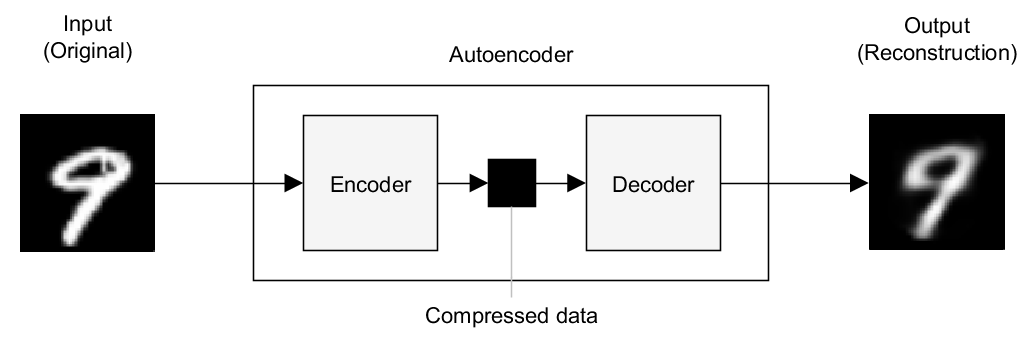
\includegraphics[scale=0.55]{images/ae_mnist.png}
	\caption{Prozess der Enkodierung und Dekodierung von Ziffern durch einen Autoencoder.}
	\label{img:ae_mnist}
\end{figure}

\subsection{Autoencoder für Bild Features}

Im vorigen Kapitel wurde veranschaulicht, wie ein Autoencoder direkt mit den Pixeln eines Bildes arbeitet. Durch eine abschließende Schicht zur Klassifizierung wird das Bild schließlich eingeordnet. Da aber in vielen Anwendungsfällen nicht direkt mit Pixeln gearbeitet werden kann, ist es wünschenswert, dass der Autoencoder stattdessen mit Features von Bildern arbeitet. Für die Extraktion geeigneter \textit{keypoints} hat sich der SIFT-Detektor bewährt, der Deskriptor hat jedoch bereits eine so kompakte Darstellung, sodass es nicht möglich ist ein tiefes Netzwerk aufzubauen. Stattdessen sollen die \textit{keypoints} als Basis für die Erstellung eines Deskriptors dienen: Dieser kodiert, wie in der Arbeit von Zhao \cite{aed2016} vorgeschlagen, die Gradienten in horizontale und vertikale Richtung der Nachbarschaft eines \textit{keypoints}. Als Größe für die Nachbarschaft wurde eine Matrix der Größe $41 \times 41$ Pixeln verwendet. Auf die Wahl der Größe wurde nicht näher eingegangen. Durch diese bestimmt sich die Größe des Feature-Vektors: Pro Richtung ergibt sich eine $39 \times 39$ Matrix und damit insgesamt ein Feature-Vektor der Länge $2 \times 39 \times 39 = 3042$. In der Arbeit wird nicht näher auf die Art der Kantendetektion eingegangen, um die Gradienten zu ermitteln. Jedoch ist es wahrscheinlich, dass ein Sobel-Operator mit einem Filterkern der Größe $3 \times 3$ verwendet wurde: Dadurch können die jeweils erste und letzte Zeile und Spalte der Bildmatrix nicht berücksichtigt werden, sodass sich eine $39 \times 39$ Matrix für die Gradienten ergibt.
Der Feature-Vektor mit 3042 Elementen bildet nun eine gute Basis, um einen mehrschichtigen Autoencoder zu entwickeln, der sukzessiv eine abstraktere Repräsentation lernt. Der von Zhao vorgeschlagene Encoder besteht aus fünf Stufen. Die erste Schicht besteht aus 3042 Neuronen um die Eingabe weiterzuleiten. Folgend werden 1024, 512, 128 und schließlich 36 Neuronen für die Kodierung verwendet. \todo{Die Neuronen jeder Schicht besitzen eine lineare Aktivierungsfunktion}. Der Decoder ist umgekehrt aufgebaut und auch die Gewichte der Kanten zwischen zwei Neuronen entsprechen ihren Pendants im Encoder.